%%%%%%%%%%      Luthesis v1.1      %%%%%%%%%%
%%% 该模板为兰州理工大学硕士学位论文模板  %%%
%%% 基于 ThuThesis LATEX Template 修改    %%%
%%% @Author Yang Guoqiang                 %%%
%%% Email estivalinp@163.com              %%%
%%%%%%%%%%%%%%%%%%%%%%%%%%%%%%%%%%%%%%%%%%%%%
\documentclass[degree=master]{thuthesis}
%\documentclass[degree=master,mangshen]{thuthesis} % 盲审格式

% 所有其它可能用到的包都统一放到这里了,可以根据自己的实际添加或者删除。
\usepackage{thuthesis}

% 定义所有的图片文件在 figures 子目录下
\graphicspath{{figures/}}

\begin{document}

	%%% 封面部分 %%%%%%%%%%%%%%%
	\frontmatter
	\thusetup{
  %******************************
  % 注意:
  %   1. 配置里面不要出现空行!!!!!
  %   2. 不需要的配置信息可以删除
  %******************************
  %
  %=====
  % 基本信息
  %=====
  secretlevel={公\hspace{1em}开},  % 密级 \hspace{1em}:水平间隔1字符
  secretyear={10}, % 保密年限
  schoolcode={10731}, % 学校代码
  classcode={TP391}, % 分类号
  stunum={123456789012}, % 学号
  submitdate={****年**月**日}, % 论文提交日期
  replydate={****年**月**日}, % 论文答辩日期
  chairman={***},  % 答辩委员会主席
  predegree={***B.E. (Lanzhou University of Technology) 2015***},  % 前置学位(英文)[获得学位等级、获得学位院校、获得学位年份]
  ereplydate={***May, 2018***}, % 答辩日期
  %=========
  % 中文信息
  %=========
  ctitle={****文章标题(请在data/cover中修改论文信息)****}, % 标题
  cdegree={硕士}, % 申请学位
  cdepartment={****学院}, % 学院
  cmajor={**计算机系统结构**}, % 学科专业
  researchdirect={**人工智能与模式识别**},  % 研究方向
  cauthor={****},  % 作者姓名
  csupervisor={***\hspace{1em}教授}, % 导师
  %=========
  % 英文信息
  %=========
  etitle={*** English Title ***}, % 标题
  edegree={***Doctor of Engineering***}, % 申请学位
  edepartment={school of ***}, % 学院
  emajor={***Computer Architecture***}, % 专业
  eauthor={***YANG Guoqiang***},  % 作者姓名
  esupervisor={Professor ***ZHAO Fuqing***}, % 导师
  % 关键词用“英文逗号”分割
  ckeywords={关键词1, 关键词2, 关键词3},
  ekeywords={Key Words 1, Key Words 2, Key Words 3}
}

% 定义中英文摘要和关键字
\begin{cabstract}
	中文摘要中文摘要中文摘要中文摘要中文摘要中文摘要中文摘要中文摘要中文摘要中文摘要
	
	中文摘要中文摘要中文摘要中文摘要中文摘要中文摘要中文摘要中文摘要中文摘要中文摘要
\end{cabstract}

% 如果习惯关键字跟在摘要文字后面,可以用直接命令来设置,如下:
% \ckeywords{\TeX, \LaTeX, CJK, 模板, 论文}

\begin{eabstract}
   Abstract Abstract Abstract Abstract Abstract Abstract Abstract Abstract Abstract Abstract
   
   Abstract Abstract Abstract Abstract Abstract Abstract Abstract Abstract Abstract Abstract
\end{eabstract}

% \ekeywords{\TeX, \LaTeX, CJK, template, thesis}

	% 如果使用授权说明扫描页,将可选参数中指定为扫描得到的 PDF 文件名,例如:
	%\makecover[scan-auth.pdf]
	\makecover
	
	% 目录
	\tableofcontents
	% 摘要
	\makeabstract
	% 插图索引
	\listoffigures
	% 表格索引
	\listoftables
	% 算法索引(可选)
	\listofalgorithms
	% 符号对照表(可选)
	\begin{denotation}[3cm]
\item[$ n $]  工件的数目
\item[$ m $]  机器的数目
\item[$ (i,j) $] 机器 $ i $ 上工件 $ j $ 的工序
\item[$ p_{j,i} $]  工件 $ j $ 在机器 $ i $ 上的加工时间
\item[$ r_j $]  工件 $ j $ 的发布日期
\item[$ d_j $]  工件 $ j $ 的交货日期
\item[$ w_j $]  工件 $ j $ 的权重
\item[$ T_0 $]  模拟退火初始温度
\item[$ R_T $]  模拟退火温度递减系数

\end{denotation}

	% 缩略词注释表(可选)
	\begin{abbreviation}

% Table generated by Excel2LaTeX from sheet 'Sheet1'

\begin{longtable}[c]{l*{3}{l}} % {c*{10}{r}} 右对齐
	\textbf{缩写} & \textbf{英文全称} & \textbf{中文全称} \vspace{6pt}\\
\endfirsthead
	\textbf{缩写} & \textbf{英文全称} & \textbf{中文全称} \vspace{6pt}\\
\endhead
\multicolumn{3}{r}{续下页}
\endfoot
\endlastfoot
    AIT   & Average Idle Time & 平均闲置时间 \\
    AMT   & Advanced Manufacturing Technology & 先进制造技术 \\
    ARPD  & Average Relative Percentage Deviation & 评价相对百分比偏差 \\
    ATSP  & Asymmetric Traveling Salesman Problem & 非对称旅行商问题 \\
    BNS   & Block-shift Neighborhood Structure & 块移动邻域结构 \\

\end{longtable}


\end{abbreviation}


	
	%%% 正文部分 %%%%%%%%%%%%%%%
	\mainmatter
	
	% 在这引入各个子章节
	\chapter{绪\hspace{1em}论}
\label{ch1:intro}

\section{引言}
LUT \LaTeX~Template: LuThesis v1.1。

该模板为兰州理工大学硕士学位论文模板,基于 ThuThesis LATEX Template 修改,Author: Yang Guoqiang,Email: estivalinp@163.com。该模板提供基本的文档元素例子,更复杂的例子请参考硕士论文:《杨国强\_车间调度问题的适应度地形及智能优化算法研究》。

注意:使用该模板时,段落之间请空一行。脚注示例\footnote{这是一个脚注。This is a footnote.}。

\section{使用展示}

\subsection{插入一幅图}

例如,图 \ref{fig:ch1:flowchat} 为制造系统中的信息流图。
\begin{figure}%[H] % use float package if you want it here
	\centering
	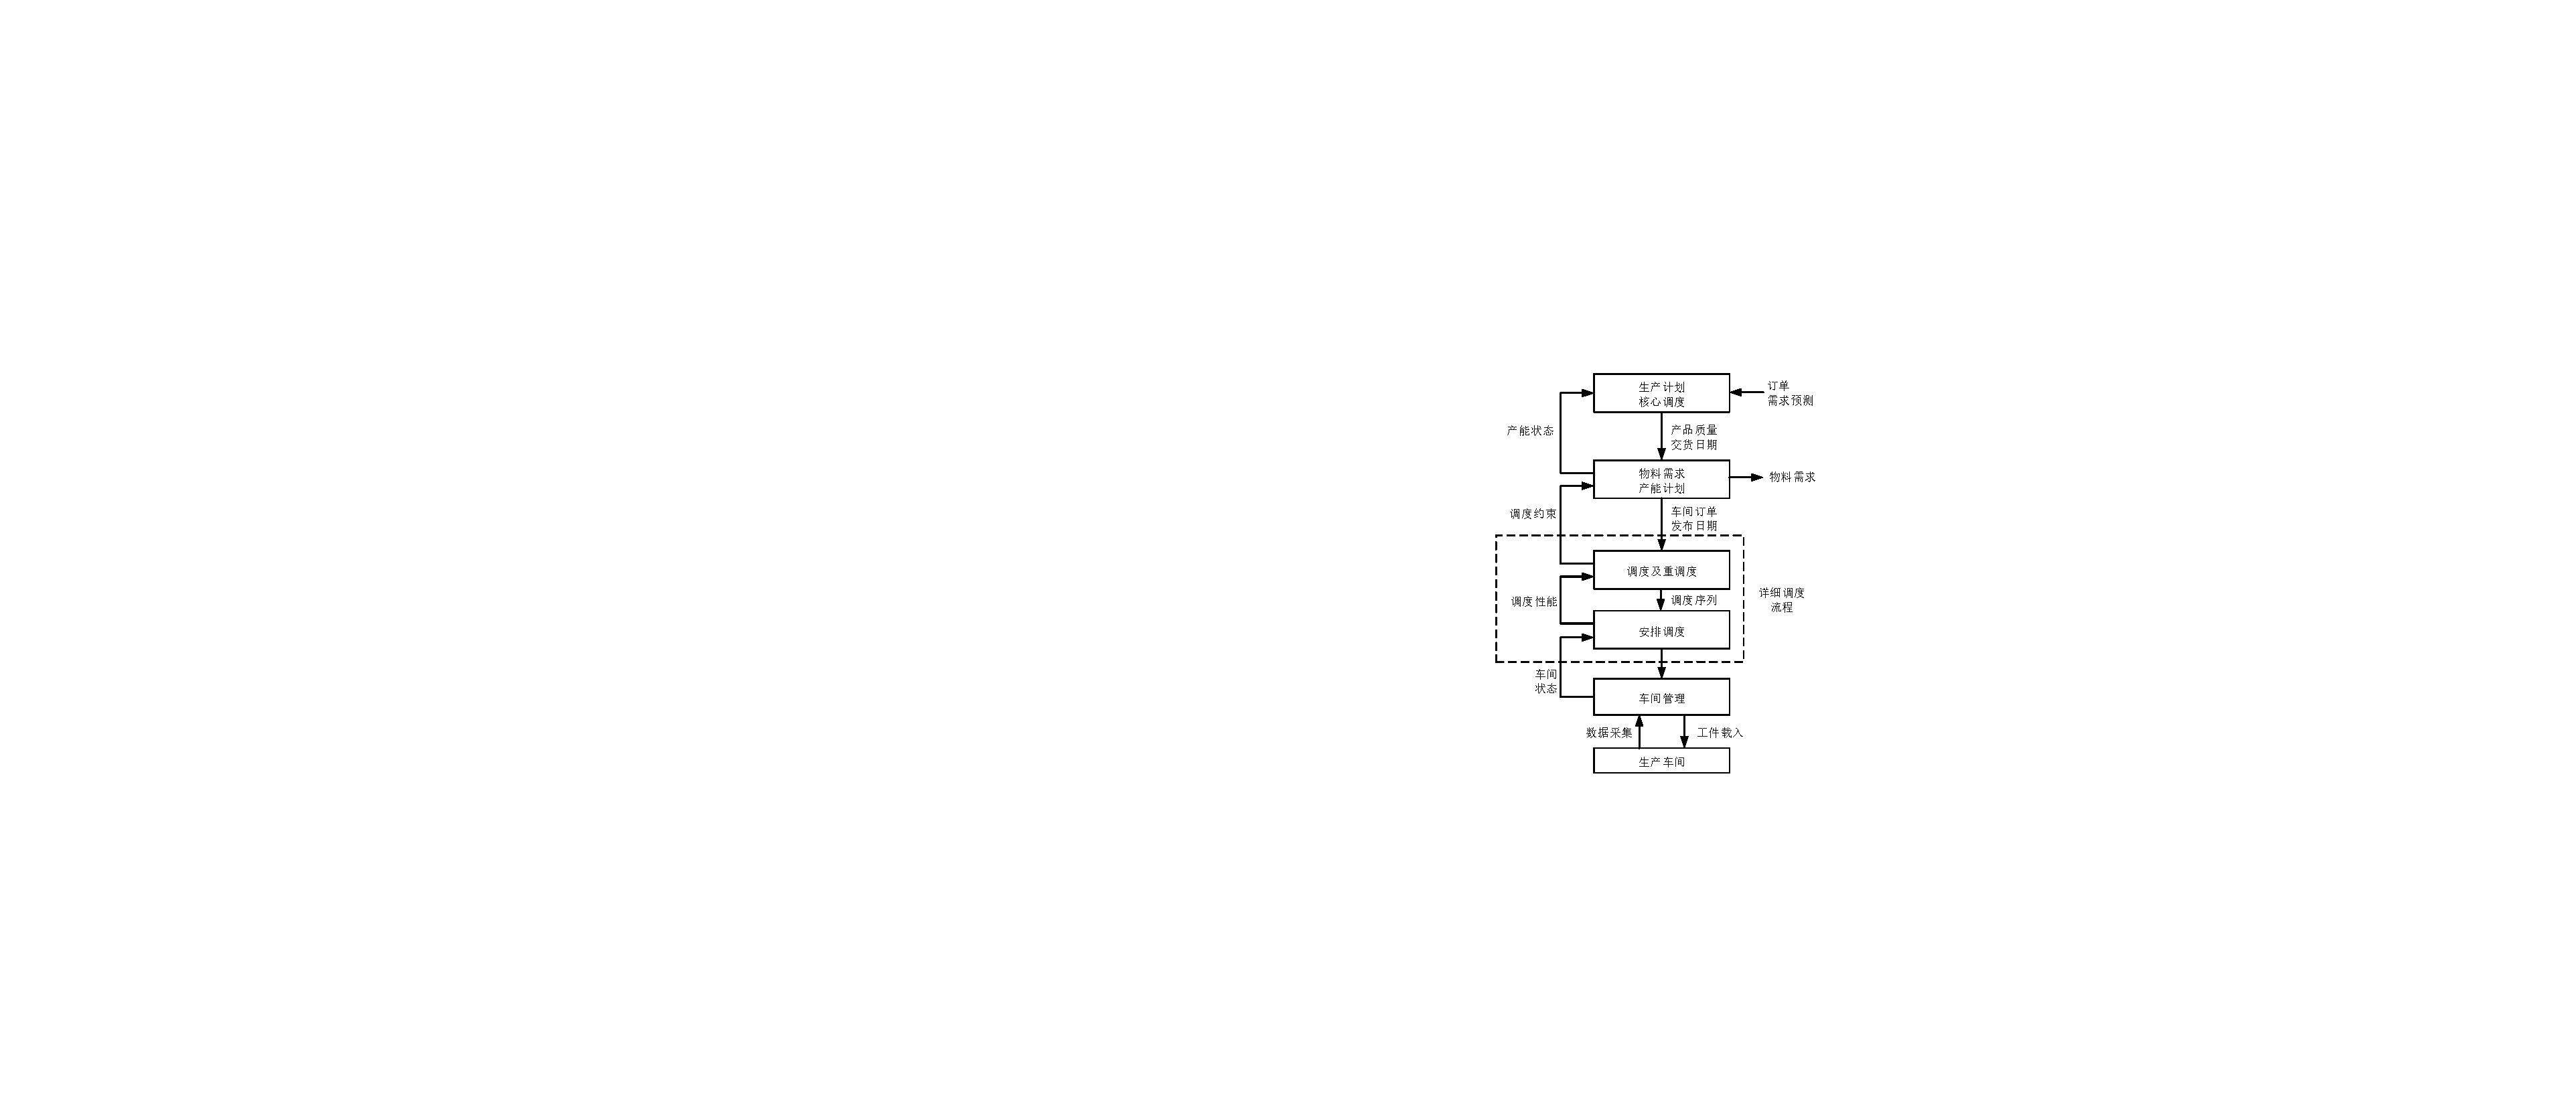
\includegraphics{fig_ch1_flowchat}
	\caption{制造系统中的信息流图}
	\label{fig:ch1:flowchat}
\end{figure}

\subsection{插入一张表}

例如,对应的映射关系如表~\ref{tab:ch2:mapping} 所示。
\begin{table}[htbp]
	\wuhao\centering
		\caption{工件序列、阶乘因子串及阶乘数之间的映射关系$(n=3)$}
		\label{tab:ch2:mapping}
		\begin{tabular}{m{4cm}<{\centering}m{4cm}<{\centering}m{4cm}<{\centering}}
			\toprule[1.5pt]
			工件序列 & 阶乘因子串 & 阶乘数(十进制形式)\\%\tabincell{c}{阶乘数\\(十进制形式)} \\
			\midrule[0.5pt]
			\{1, 2, 3\} & \{0, 0, 0\} & 0\\
			\{1, 3, 2\} & \{0, 1, 0\} & 1\\
			\{2, 1, 3\} & \{1, 0, 0\} & 2\\
			\{2, 3, 1\} & \{1, 1, 0\} & 3\\
			\{3, 1, 2\} & \{2, 0, 0\} & 4\\
			\{3, 2, 1\} & \{2, 1, 0\} & 5\\
			\bottomrule[1.5pt]
		\end{tabular}
\end{table}

\subsection{插入一个行间公式}

例如,最后一台机器上的两个相邻工件完成时间之差 $d_{j-1,j}$ 可由公式(\ref{equ:chap1:distence})算得。

注意,模板中正文与begin{equation}之间不能存在空行,{\heiti 这是正文中的黑体}。
\begin{equation}
	\label{equ:chap1:distence}
	\begin{aligned}
	d_{j-i,j}=C_{i,m}-C_{j-i,m}&=\sum_{k=1}^{i}{p_{j,k}}-\min\limits_{1 \leq i \leq m}\big(\sum_{k=1}^{i-1}{p_{j,k}}+\sum_{k=i+1}^{m}{p_{j-1,k}}\big)\\
	&=\max\limits_{1 \leq i \leq m}\big(\sum_{k=1}^{m}{p_{j,k}}+\sum_{k=1}^{i-1}{p_{j,k}}-\sum_{k=i+1}^{m}{p_{j-1,k}}\big)\\
	&=\max\limits_{1 \leq i \leq m}\big(\sum_{k=1}^{m}{p_{j,k}}-\sum_{k=i+1}^{m}{p_{j-1,k}}\big)
	\end{aligned}
\end{equation}

\subsection{插入一个算法}

例如,算法 \ref{alg:ch2:encoding} 给出了阶乘数的详细编码过程。

\begin{myAlgorithm}
	\setstretch{1}
    \caption{阶乘数编码算法} %\strut
    \label{alg:ch2:encoding}
    \KwIn{Job permutation $\pi=\{J_1,J_2,\cdots,J_{j-1},J_j,\cdots,J_n\} $\;}
    \KwOut{Natural number $ N_F $\;}
    \textbf{Initialize: }$ D_F=\{0,1,\cdots,n-1\} $, $ P=\{1,2,\cdots,n\} $, $ F=\varnothing $, $  N_F=0 $\;
    \For {$j \gets 1;j \leqslant n;j \ne i$}
    {
		 \algolines{$ index \gets Find(P[index]==J_i) $}{Find the first position index from left to right in $ P $ which makes $ P[index] $ equal to $ J_i $.}
		 $F[i] \gets D_F [index]$\;
		 remove $ P[index] $ from $ P $\;
		 $ N_F \gets N_F+F[i] \times D_F [n-i+1]! $\;
    }
    \Return{$ N_F $}
\end{myAlgorithm}

\subsection{定理及证明}

本文使用Markov模型对HILS的收敛性进行分析。本文使用的依概率收敛定义如下:

\begin{definition}
	(依概率收敛\textsuperscript{[160]})设 $ \{x(t),t=0,1,2 \cdots \} $ 为基于种群的随机算法产生的种群随机序列。称随机序列 $ \{x(t)\} $ 依概率弱收敛于全局最优,当且仅当:	
	\begin{equation}
		\label{equ:chap5:equation1}
		\lim_{t \to +\infty}P\{x(t) \cap B^* \neq \varnothing\}=1
	\end{equation}
	
	\noindent 其中 $ B^* $ 为优化问题的全局最优解。
\end{definition}
	
\begin{nature}
	对于不包含SHADE中选择算子的HILS,其种群空间 $ \varPhi^m $ 的所有状态(种群)都是连通的。对于所有状态 $ X,Y \in \varPhi^m $,从 $ X $ 到 $ Y $ 的一步转移概率大于0。即:
	\begin{equation}
		\label{equ:chap5:nature1}
		P\{A^0 \cdot L^0 \cdot P^0 (X)=Y\}>0. 
	\end{equation}
\end{nature}

\begin{theorem}
	\label{sec:theorem}
	假设 $ \{x(t),t=0,1,2 \cdots\} $ 为HILS迭代过程中的种群序列,则 $ \{x(t),t=0,1,2 \cdots\} $ 能依概率收敛到全局最优。
\end{theorem}

\begin{proof}
	对于不包含SHADE中选择算子的HILS,仅存在三个算子:扰动算子 $ P^0 $,局部搜索算子$  L^0 $ 和接受准则算子 $ A^0 $。又因为 $ e^{- \Delta f / T_G}>0 $,所以:
	\begin{equation}
		\label{equ:chap5:proof1_3}
		e^{- \Delta f/T_G}  \cdot \sum_{Z \in \varPhi^m}P\{L^0 \cdot P^0 (X)=Z\} \cdot P\{A^0 (X,Z)=Y\}>0.
	\end{equation}
	
	\noindent (这是不缩进的一段)即,对于不包含SHADE中选择算子的HILS而言,从任意状态 $ X $ 到任意状态 $ Y $ 的一步转换概率大于0。因此,对于没有选择算子的HILS,所有种群状态都是连续的。\hfill $ \square $
\end{proof}

\subsection{条、款的使用}

\begin{enumerate}
	\item 第一条第一条第一条第一条第一条第一条第一条第一条第一条第一条第一条第一条第一条第一条第一条第一条第一条第一条第一条第一条第一条第一条第一条第一条第一条第一条第一条第一条第一条第一条第一条第一条第一条第一条第一条第一条第一条第一条第一条。
	\begin{itemize}[itemsep=0ex,partopsep=0pt,parsep=0ex,topsep=6bp,labelsep=10pt]
		\item 第一款第一款第一款第一款第一款第一款第一款第一款第一款第一款第一款第一款第一款第一款第一款第一款第一款;
		\item 第二款第二款第二款第二款第二款第二款第二款第二款第二款第二款第二款第二款第二款第二款第二款第二款第二款;
		\item 第三款第三款第三款第三款第三款第三款第三款第三款第三款第三款第三款第三款第三款第三款第三款第三款第三款。
	\end{itemize}
	\item 第二条第二条第二条第二条第二条第二条第二条第二条第二条第二条第二条第二条第二条第二条第二条第二条第二条第二条第二条第二条第二条第二条第二条第二条第二条第二条第二条第二条第二条第二条第二条第二条第二条第二条第二条第二条第二条第二条第二条。
	\item 第三条第三条第三条第三条第三条第三条第三条第三条第三条第三条第三条第三条第三条第三条第三条第三条第三条第三条第三条第三条第三条第三条第三条第三条第三条第三条第三条第三条第三条第三条第三条第三条第三条第三条第三条第三条第三条第三条第三条。
\end{enumerate}

\section{本论文的主要研究内容及创新之处}
***

\section{本论文的组织安排}
***

	\chapter{第二章标题}
\label{ch2:keymethods}

\section{第一节标题}
\label{ch2:sec1}
***
\subsection{第一小节标题}
***
\section{本章小结}
***
	
	%%% 其它部分 %%%%%%%%%%%%%%%
	\backmatter
	
	%% 参考文献(当前版本不完善)
	% 注意:至少需要引用一篇参考文献,否则下面两行可能引起编译错误。
	% 如果不需要参考文献,请将下面两行删除或注释掉。
	% 数字式引用
	%\bibliographystyle{thuthesis-numeric}
	% 作者-年份式引用
	% %\bibliographystyle{thuthesis-author-year}
	%\bibliography{ref/refs}
	
	%% 总结 %%%%%%%%%%%%%%%
	\begin{conclusion}

****

\end{conclusion}


	
	%% 参考文献 %%%%%%%%%%%%%%%(该版本还需手动输入,将在以后版本中完善)
	\begin{references}
  \begin{publications}[itemsep=0.5ex,partopsep=0pt,parsep=0ex,topsep=0bp,labelsep=6pt,listparindent=0pt]
\item 赵付青. 可重构制造系统:Holonic制造系统建模、优化与调度方法 [M]. 国防工业出版社, 2012.
\item 周佳军, 姚锡凡. 先进制造技术与新工业革命 [J]. 计算机集成制造系统, 2015, 21(8): 1963-1978.
\item Pinedo M L. Scheduling: theory, algorithms, and systems [M]. Springer, 2016.
\item 赵付青, 宋厚彬. 智能制造关键使能技术-动态HOLONIC制造系统建模技术重构方法及优化理论 [M]. 电子工业出版社, 2017.
\item Smith T, Husbands P, O'shea M. Fitness landscapes and evolvability [J]. Evolutionary computation, 2002, 10(1): 1-34.
\item 王莽. 智能优化算法表型空间的动态行为学分析与应用 [D]; 中国科学技术大学, 2017.
\item Shao W, Pi D. A self-guided differential evolution with neighborhood search for permutation flow shop scheduling [J]. Expert Systems with Applications, 2016, 51: 161-176.
\item Johnson, David S. Computers and intractability [M]. W.H. Freeman, 1979.
	\end{publications}
\end{references}


	
	%% 致谢 %%%%%%%%%%%%%%%
	\cleardoublepage % open right 格式,即下一节在奇数页,这会导致正常出现的空白页
	\begin{acknowledgment}%{\DejaSans 😋}

****

还要向在百忙之中评审本论文的各位专家、教授们表示衷心的感谢!


\end{acknowledgment}



	
	%% 附录 %%%%%%%%%%%%%%%
	\begin{appendix}
	
		% 附录A
		\cleardoublepage
		\chapter{攻读学位期间的研究成果及发表的学术论文}
%在攻读硕士学位期间共发表论文1篇,其中核心期刊*篇,投稿SCI/EI收录*篇。
\begin{publications}
\item Zhao F, Yang G, Zhang Y, et al. The Convergence and Optimization Performance of the Simplified Artificial Fish School Algorithm [C]. In: The 4th International Conference on Applied Science and Engineering Innovation (ASEI), 2018: Accepted.
\end{publications}
		
		% 附录B(可选)
		\cleardoublepage
		\chapter{附录B标题(可选)}

	
	\end{appendix}

\end{document}
